\chapter{Result From Flight Data}\label{ch:FlightResult}

This chapter is divided into three main sections. Firstly, the
algorithm's convergence and consistency was analyzed. Secondly, the
accuracy of the algorithm is examined by comparing to ground truth
data. The third section summarized test results for tuning the
algorithm for better accuracy and efficiency. The forth section
present the advantage of using IMU data. The fifth section outline
the inadequacies of the CC\_EKF\_SLAM algorithm identified.

To test the performace of CC\_EKF\_SLAM algorithm, 4 segments of video
were selected from the test flight video, and 400 frames were
processed in each piece. The filter initialized 40 features at the
first frame, and maintain the tracked features amount at this number
by initializing new features when existing features moved out of FOV.

Since all parameters are tracked in camera frame, their value is 
different when viewed from a fixed point in world frame. Therefore, all 
parameters are converted back to world frame before plotting. 

\section{Convergence and Consistency}

\subsection{Convergence and Tracking}
Among the feature parameters, the feature initialization point were
initialized to the zero which is the origin of the camera centric
coordinate. $\phi$ and $\theta$ were calculated directly from the
feature position on image plane, have high accuracy and don't require
convergence. The only parameter that goes through a converging process
is the features' inverse depth $\rho$, which were initialized to 0.1
for all features. Figure \ref{fltfig:1} shows the $1/\rho$ plot for
video segment1 over 200 frames. The depth estimators went through
rapid changes for several frames after their initialization. Within
approximate 20 frames, most estimtors settles to a stable value. The
estimated features distance ranged from 400 meters to about 1500
meters, confirming the algorithm's capability for estimating features
at great distance. On the other hands, some features take a long time
to settle, such as feature 9, 27, ??, while some other never settled,
such as 12 and 20.
% is the non and slowly settled feature has any character in its
% pattern? ie. is a line feature, instead of corner? A outlier filter
% should be in place to get rid of the poor features (future work).

\begin{figure}[h]
\centering
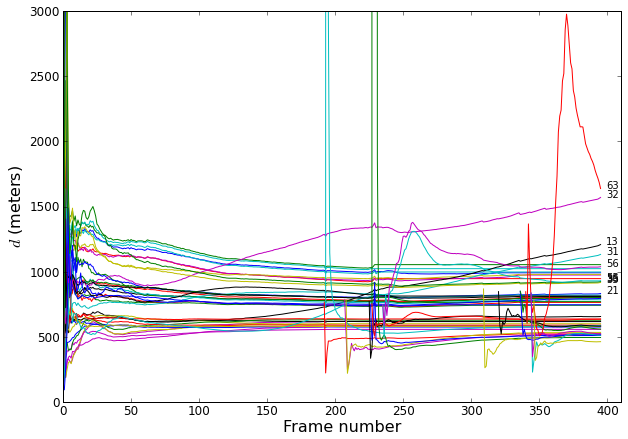
\includegraphics[width=10cm, keepaspectratio=true]{./Figures/fltfig/cut1/Figure10.png}
\caption{Inverse Depth Convergence}
\label{fltfig:1}
\end{figure}

Although the features initialization point $[x_i, y_i, z_i]$, and the
deviation-elevation angle pair $[\phi, \theta]$ did not go through a
converging stage, they do get updated and converted into the new
camera coordinate using the estimated camera motion at every
iteration. As a result, the accuracy of these parameters varies.
Ideally, the coordinates should converge to a fixed value. However,
the plot indicates a variation as the vehicle travels along. Figure
\ref{fltfig:2} shows the tracking of these parameters over the entired
processed frames.
These parameters were stable for about 200 frames. As soon as any
feature was deleted from the filter and new features added, the
paramters of the feature after being converted into world
frame start to drift. In \ref{fltfig:2} the deletion of old feature is
marked by a vertical gray dash line. It shows that the parameters of
the deleted feature start to drift right after that line. The $y_i$
and $z_i$ are most affected. The behavior is caused by the estimated
error in the SUAS localization. In order to compensate the error in
localization(Figure \ref{fltfig:4}), the algorithm made adjustment on the
estimate of  features parameters so that the combinational result
agrees with the measurement. On the other hand, features mapping is
not affected too much by the error in localization. Because their
parameters are transformed in each iteration to the new camera frame
using the estimated SUAS motion which carries the error. As long as
their paramters are updated together with the estimated motion on that
iteration, and transformed back to the world frame using the same
estimated motion, the final result of features location in world frame
is inaffected by the error in the SUAS localization. However, for
feature removed from the filter, their parameters are no longer
updated, therefore revealing the error in SUAS localization. 

\begin{figure}[h]
\centering
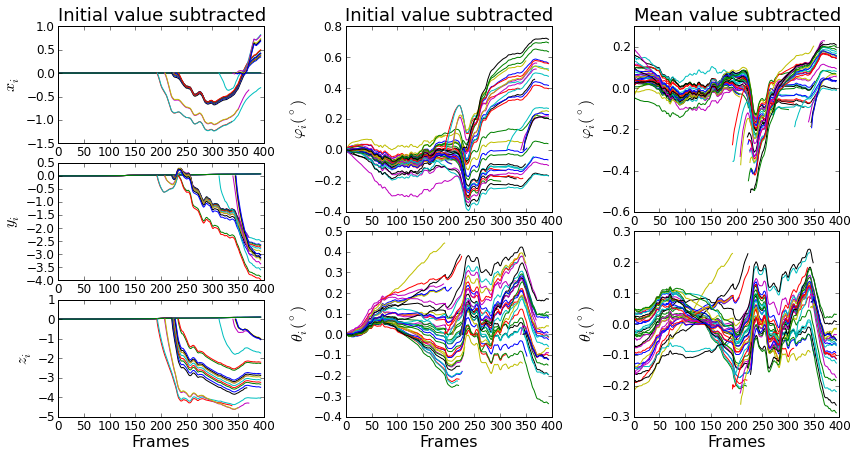
\includegraphics[width=12cm, keepaspectratio=true]
{./Figures/fltfig/cut1/Figure20.png}
\caption{Feature parameters tracking}
\label{fltfig:2}
\end{figure}

A EKF system becomes inconsistent when the variance of state vector
element becomes too small and forbid an effective update. In addition,
the uncertainty of the SUAS position should increases as it move away
from the origin. To examine the consistency of the CC\_EKF\_SLAM
algorithm, the variance of all state vectors for all procesed frames
were extracted and plotted in figure \ref{fltfig:3}. The two plots on
the left shows the variance of world frame position and orientation in
camera frame. The three plots on the right show the variance of
feature parameters. The variance of world frame position increases
with iterations. On the other hand, world frame orientation decreases
with iterations. Especially the orientation in Y and Z axis remain
below 5e-7 for the most time. For feature parameters, all variance
decreases with iterations, and their value is very small. 
\begin{figure}[h]
\centering
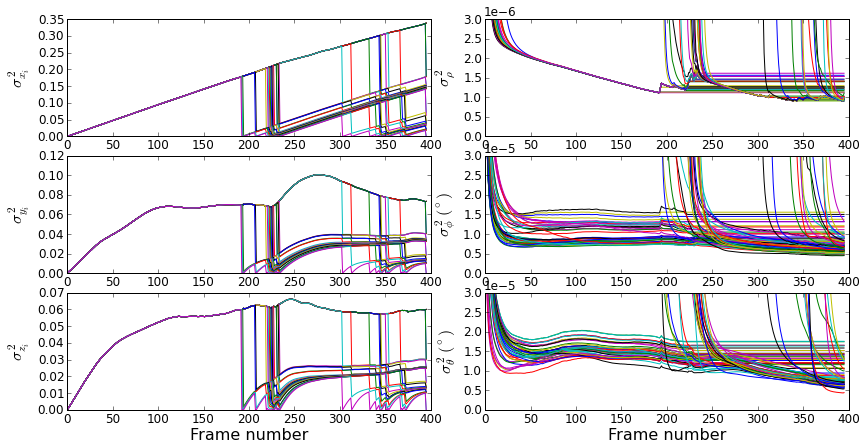
\includegraphics[width=12cm, keepaspectratio=true]
{./Figures/fltfig/cut1/Figure40.png}
\caption{State vector variance}
\label{fltfig:3}
\end{figure}

To see how variance affect the correction the filtered made on the
state vector, the correction applied each iteration were plotted ni
figure \ref{fltfig:4}. The $1^{st}$ column shows the correction on
world frame position in camera frame. The $2^{nd}$ column shows the
correction on feature initialization coordinate in camera frame. The
$3^{rd}$ column shows the correction on features parameters $\rho$,
$\phi$ and $\theta$. It can be observed that world frame position on Y
and Z component receive more correction than the X component, despite
their variance is smaller than the X axis. Similarly, feature
parameter $\theta$ and $\phi$ receive more correction than $\rho$
despite their variance is smaller than the variance of $\rho$.
Secondly, there is a strong inverse correlation between the Y and Z
component of feature initialization position and the world frame
position on Y and Z axis. Similarly, $\phi$ is correlated to world
frame position Z component, $\theta$ is correlated to the world frame
position Y component.

\begin{figure}[h]
\centering
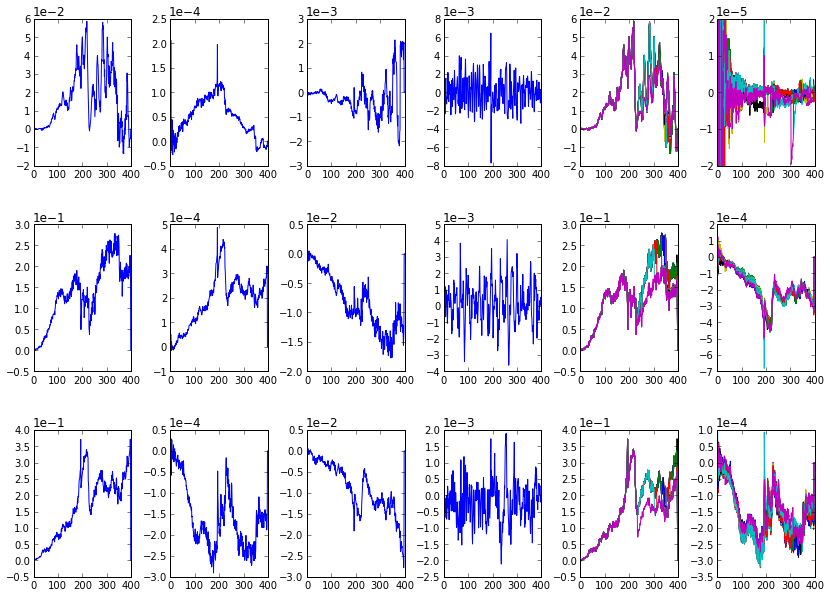
\includegraphics[width=12cm, keepaspectratio=true]
{./Figures/fltfig/cut1/Figure112.png}
\caption{State Vector Corrections}
\label{fltfig:4}
\end{figure}

\begin{figure}[h]
\centering
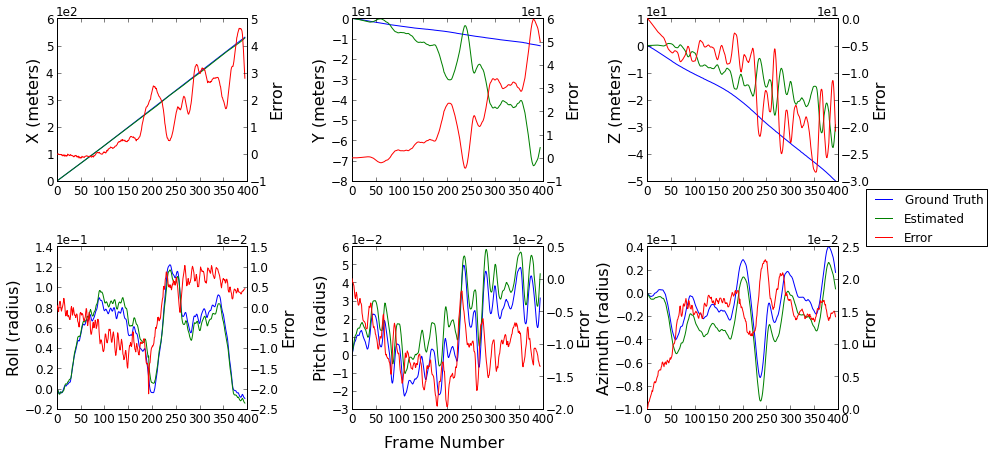
\includegraphics[width=12cm, keepaspectratio=true]
{./Figures/fltfig/cut1/Figure30.png}
\caption{Estimates of SUAS position and orientation}
\label{fltfig:4}
\end{figure}

\begin{figure}[h]
\centering
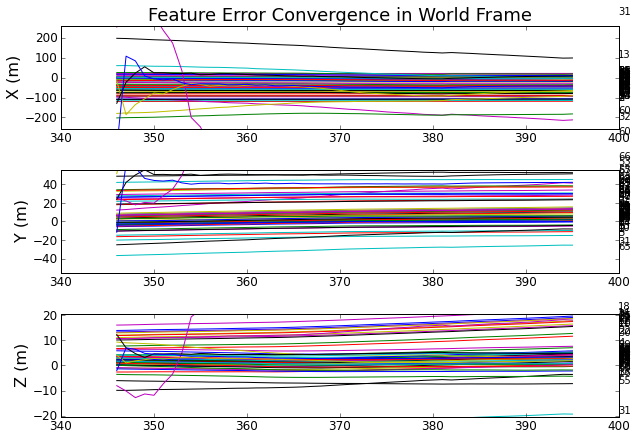
\includegraphics[width=12cm, keepaspectratio=true]
{./Figures/fltfig/cut1/Figure50.png}
\caption{Feature position error}
\label{fltfig:5}
\end{figure}

% is the drift still correlated with UAS? Stop plotting those features
% that's out of FOV to see what happen.
Comparing the pattern of the drift, it is highly 
correlated to the aircraft pitch and yaw rotation (figure?). The 
significant of the drift is measured by the maximum drift seen 
throughout the 200 processed frame, and are listed below (table?). The 
maximum drift is defined by:


%%% Local Variables:
%%% mode: latex
%%% TeX-master: "thesis"
%%% End:
